\documentclass[UTF8,a4paper,11pt,fontset=fandol]{ctexart}
\usepackage[margin=2.35cm]{geometry}
\usepackage{amsmath,amssymb,booktabs,longtable,graphicx,float,array,tabularx}
\usepackage[dvipsnames]{xcolor}
\usepackage{caption,subcaption,fancyhdr,enumitem}
\usepackage[section]{placeins}
\usepackage{needspace}
\usepackage[unicode,colorlinks=true,linkcolor=MidnightBlue,citecolor=MidnightBlue,urlcolor=MidnightBlue]{hyperref}
\usepackage{bookmark}
\usepackage{xurl}
\hypersetup{pdftitle={基于H\&E组织学图像的人肝空间转录组预测：统一高表达基因基准与多尺度集成实验报告},pdfauthor={庹力元},pdfsubject={东南大学生命科学与技术学院；学号59S2311}}
\setlength{\headheight}{15pt}
\pagestyle{fancy}\fancyhf{}
\fancyhead[L]{\small 人肝空间转录组预测实验报告}
\fancyhead[R]{\small 庹力元\quad 59S2311}
\fancyfoot[C]{\thepage}
\setlist{nosep,leftmargin=2em}
\renewcommand{\arraystretch}{1.15}
\captionsetup{font=small,labelfont=bf}
\graphicspath{{figures/}}
\newcommand{\HE}{H\&E}
\newcommand{\PCC}{\operatorname{PCC}}
\newcommand{\MAE}{\operatorname{MAE}}
\newcommand{\code}[1]{\nolinkurl{#1}}

\setlength{\parindent}{2em}
\setlength{\parskip}{0.25em}
\emergencystretch=1.5em
\renewcommand{\figurename}{图}
\renewcommand{\tablename}{表}
\captionsetup{labelsep=quad}
\newcolumntype{Y}{>{\raggedright\arraybackslash}X}

\begin{document}
\hypersetup{pageanchor=false}
\begin{titlepage}\centering
\vspace*{1.2cm}
{\Large 东南大学生命科学与技术学院\par}
\vspace{1.5cm}
{\Huge\bfseries 实验研究报告\par}
\vspace{1.1cm}
{\LARGE\bfseries 基于\HE 组织学图像的\par 人肝空间基因表达预测\par}
\vspace{.7cm}
{\Large 多方法比较与多尺度集成模型研究\par}
\vspace{1.6cm}
\begin{tabular}{rl}
姓\quad 名：& 庹力元\\[.5em]
学\quad 号：& 59S2311\\[.5em]
学\quad 院：& 东南大学生命科学与技术学院\\[.5em]
学位背景：& 生物、计算机双学位学士\\[.5em]
修订日期：& 2026年9月19日
\end{tabular}
\vfill
\begin{minipage}{.85\textwidth}\small
研究对象为 GSE240429 中同一供体的四张人肝连续切片。通过组织图像预测每个测量位置的 200 个高表达基因，比较已有方法的适配实现，并分析多尺度图像输入与模型集成的作用。
\end{minipage}
\end{titlepage}
\pagenumbering{Roman}\hypersetup{pageanchor=true}
\section*{摘要}\addcontentsline{toc}{section}{摘要}
苏木精--伊红（hematoxylin and eosin，\HE）染色图像能够反映细胞形态和组织结构，但不直接提供基因表达信息。本研究以人肝组织为对象，研究能否利用配对的组织图像和空间转录组数据，学习从局部形态到空间基因表达的映射，并比较不同预测方法在相同测试条件下的表现。

实验使用 GSE240429 的四张连续切片，其中两张用于训练，一张用于验证，一张用于测试。仅根据训练集平均表达量选择 200 个高表达基因（HEG200），同时评价其中表达量最高的 50 个基因（HEG50）。在实现 ST-Net、BLEEP、ResSAT、GenAR 和 Stem 的人肝适配版本后，构建三尺度图像回归模型 ContextFusion，并将不同随机种子和训练配置的六个模型进行加权集成。模型选择依据验证集表现，测试指标为逐基因 Pearson 相关系数（PCC）的平均值及平均绝对误差（MAE）。

在测试切片 D1 上，六模型集成的 HEG200 和 HEG50 PCC 分别为 0.2343 和 0.3180，较本地 ST-Net 适配模型分别提高 0.0872 和 0.1202。参数量与训练流程一致的输入视野对照显示，三尺度输入较单视野输入分别提高 PCC 约 0.0236 和 0.0228。六模型集成进一步改善了基础三模型集成中 151 个基因的相关性，HEG200 平均 PCC 增加 0.0042。结果表明，组织上下文与端到端图像特征学习有助于人肝空间表达预测，模型集成能够提供进一步的相关性增益。该结论适用于当前同供体跨切片任务，尚需独立供体数据验证。

\noindent\textbf{关键词：}空间转录组；组织学图像；高表达基因；多尺度学习；模型集成
\clearpage\tableofcontents
\clearpage\listoffigures
\clearpage\pagenumbering{arabic}

\section{引言}
空间转录组技术在组织切片的不同位置测量 RNA，使研究者能够观察基因表达在组织中的分布。\HE 染色则以较低成本呈现细胞和组织形态。如果能够从图像中预测与形态相关的表达变化，便可为组织结构与分子表型的关联分析提供补充信息。

已有方法分别采用局部卷积回归、图像与表达的对比学习、空间注意力、自回归生成和条件扩散等技术\cite{stnet,bleep,ressat,genar,stem}。这些研究的组织类型、预测基因及数据处理方式并不相同。为评价它们在同一人肝任务上的适用性，本研究统一切片划分、基因集合和测试指标，并在此基础上设计融合多个图像视野的回归模型。

本研究围绕三个问题展开：第一，现有方法在人肝高表达基因预测中表现如何；第二，在其他训练条件尽量一致时，扩大图像视野能否改善预测；第三，组合多个已训练模型能否进一步提高预测相关性。实验依次包括已有方法比较、图像视野对照和模型集成分析。主要结果见第\ref{sec:results}节，辅助配置和补充实验见附录。

\section{数据与预测任务}
\subsection{样本来源与基本数据单位}
数据来自 GEO 数据集 GSE240429，其关联研究为 Andrews 等对健康和原发性硬化性胆管炎人肝免疫景观的分析\cite{andrews,geo}。本实验使用其中健康供体 C73 的四张连续切片，\HE 图像取自 GEO，表达矩阵和空间位置文件采用 BLEEP 作者整理的版本\cite{bleep}。原始生物学研究与 BLEEP 预测方法分别作为数据来源和方法来源引用。

空间转录组中的一个测量位置通常称为 \textit{spot}。本研究每个 spot 包含三类信息：在组织图像中的二维坐标、以该坐标为中心的染色图像，以及相应的基因计数向量。spot 是空间测量单位，不等同于单个细胞；不同位置还可能因组织结构而存在相关性。

训练时将每个位置的图像与 RNA 表达配对，学习图像到表达的映射。预测时输入图像和位置坐标，输出 200 个基因的表达向量，再按原始坐标排列成空间表达图。D1 共有 2265 个位置，因此最终预测为 $2265\times200$ 的矩阵，行对应位置，列对应预先确定的基因。输出的具体表达单位在第\ref{sec:target}节定义。

\subsection{训练、验证与测试划分}
按照完整切片划分数据，而非将同一切片的图块随机分配到不同集合。训练集用于更新模型参数；验证集用于选择超参数、模型保存时点和集成权重；测试集用于计算最终预测误差。表\ref{tab:split}列出具体分配。

\begin{table}[H]\centering
\caption{数据集划分及各切片用途}\label{tab:split}
\begin{tabular}{lrrl}\toprule
切片&位置数&样本编号&用途\\\midrule
C73\_A1&2378&GSM7697868&训练\\
C73\_B1&2349&GSM7697869&训练\\
C73\_C1&2277&GSM7697870&验证、模型选择\\
C73\_D1&2265&GSM7697871&测试\\\bottomrule
\end{tabular}
\end{table}

训练集共 4727 个位置。图\ref{fig:data}展示四张切片的组织形态。由于它们来自同一供体，本实验评价的是同供体跨切片预测能力。D1 在项目开发阶段已被多次评价，属于固定开发测试集，而非全新的外部验证队列。

\begin{figure}[htbp]\centering
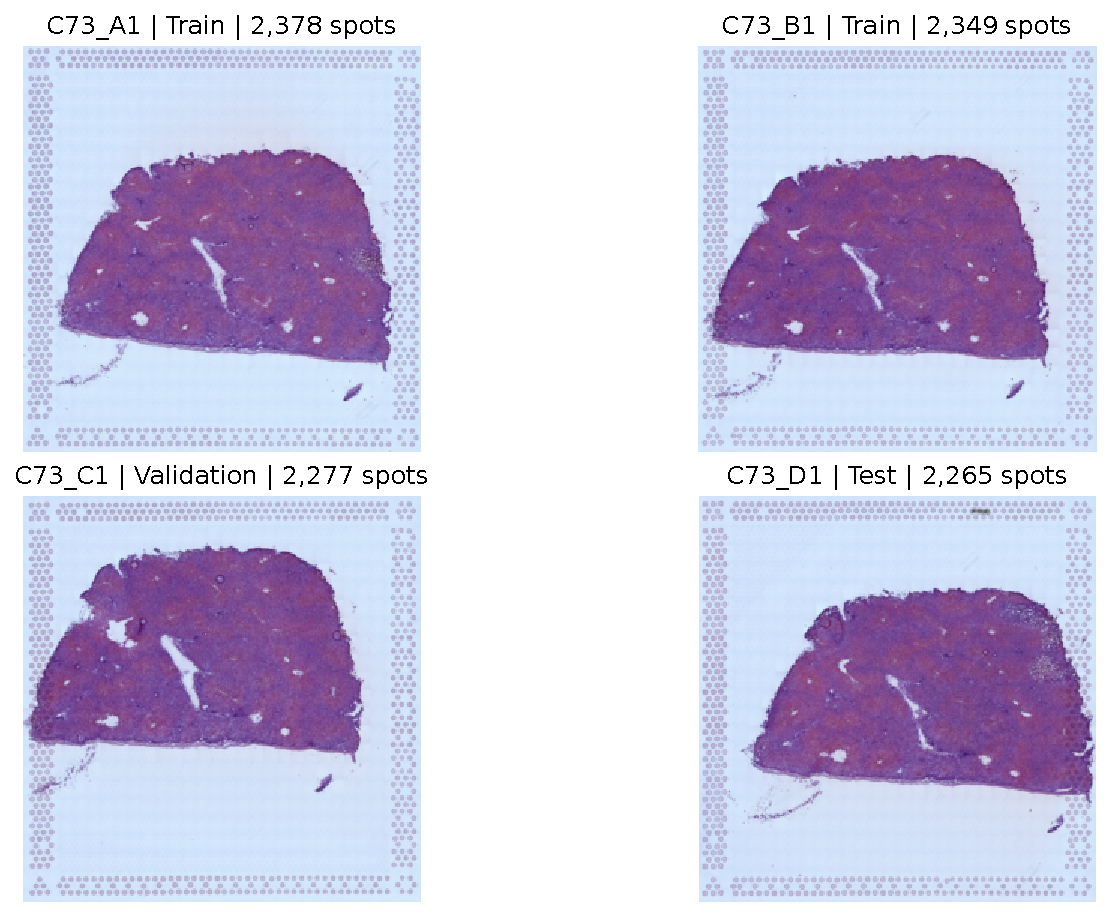
\includegraphics[width=.86\textwidth]{data_overview.pdf}
\caption[人肝切片及数据集划分]{GSE240429 四张人肝切片的组织学图像。A1、B1 用于训练，C1 用于模型选择，D1 用于测试。图中为 GEO 原始图像的缩略图，用于展示组织形态与染色情况；各图显示尺寸不代表实际组织面积。}\label{fig:data}
\end{figure}


\subsection{高表达基因的选择}
为使研究聚焦于表达量较高的基因，先使用 A1+B1 的全转录组计数计算标准化表达，再按基因的训练平均表达量排序。设 $c_{ig}$ 为位置 $i$ 上基因 $g$ 的计数，$\mathcal G_{\rm all}$ 为全转录组基因集合，则
\begin{equation}
z_{ig}=\log\left(1+10^4\frac{c_{ig}}{\sum_{h\in\mathcal G_{\rm all}}c_{ih}}\right),\qquad
\bar z_g=\frac{1}{n_{\rm train}}\sum_{i\in\rm train}z_{ig}.
\end{equation}
其中，除以总计数是为了减小不同位置捕获 RNA 总量的影响；乘以 $10^4$ 统一尺度，取自然对数则压缩高计数的数值范围。按 $\bar z_g$ 降序取前 200 个基因，定义为 HEG200；其中前 50 个定义为 HEG50。HEG 为 highly expressed genes 的缩写，表示高表达基因。本研究未按测试相关性或表达方差重新选基因。

重复基因符号保留首次出现，空名称剔除。核糖体和线粒体基因按相同标准参与排序，最终包含 47 个 RPL/RPS 基因和 9 个 MT- 基因。图\ref{fig:panel}显示，HEG200 在训练集中的最低检出率为 94.20\%，中位数为 98.48\%。这一集合具有较高的表达覆盖度，适合用于检验形态与相对表达的关系。

\begin{figure}[htbp]\centering
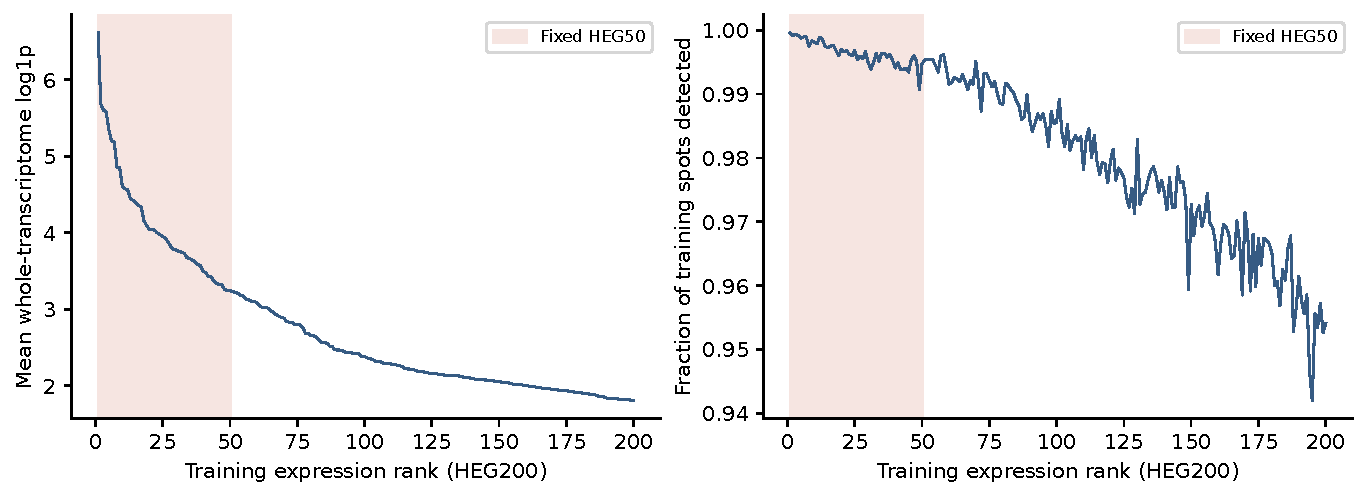
\includegraphics[width=\textwidth]{gene_panel.pdf}
\caption[高表达基因的训练表达量与检出率]{HEG200 的训练集统计。左图为按平均表达量排列的基因，右图为相同顺序下的检出率，即计数大于零的训练位置比例。阴影标出 HEG50，两个集合均只根据 A1+B1 确定。}\label{fig:panel}
\end{figure}

所有方法使用同一基因集合及列顺序。HEG50 始终是 HEG200 中预先指定的子集；计算 HEG50 指标时，仅选择相应列，不再重新归一化。具体基因名称和训练统计随报告的复现材料保存。

\subsection{预测目标及不同方法的输出转换}\label{sec:target}
本研究预测的是所选 200 个基因内部的相对表达，而非绝对 RNA 分子数。对每个位置，将这 200 个基因的计数总和归一化至 $10^4$，再取自然对数：
\begin{equation}\label{eq:target}
y_{ig}=\log\left(1+10^4\frac{c_{ig}}{\sum_{h\in\mathcal G_{200}}c_{ih}}\right),\quad g\in\mathcal G_{200}.
\end{equation}
例如，某基因计数为 20，该位置 200 个基因总计数为 2000，则目标值为 $\log(101)\approx4.615$。不同位置的同一基因均按式\eqref{eq:target}计算，模型据此学习它在空间上的相对变化。

选基因时使用全转录组总计数，以确定基因在训练组织中的表达排名；预测目标使用所选基因总计数，使仅输出 200 个基因的方法能够在同一单位下评价。ContextFusion 直接学习式\eqref{eq:target}，预测结果不再二次归一化。已有方法若输出计数，则将预测计数按相同方式变换；若输出全转录组归一化后的 log 表达，则先用指数逆变换恢复非负丰度，再以预测的 200 基因丰度总和归一化。转换分母取自预测结果，不使用测试 RNA 的总量。

所有主结果的参照值均来自式\eqref{eq:target}，不进行主成分分析（PCA）重建或邻域平均。ResSAT 适配在训练目标内部使用 PCA，预测后反投影回基因空间，但最终仍与同一未重建参照值比较。由此区分模型内部处理与最终评价目标。

\subsection{评价指标及其含义}
主要指标为 Pearson 相关系数（PCC）。对于每个基因，将它在 D1 的 2265 个实测值与 2265 个预测值配对，计算
\begin{equation}
r_g=\frac{\sum_i(y_{ig}-\bar y_g)(\hat y_{ig}-\overline{\hat y}_g)}
{\sqrt{\sum_i(y_{ig}-\bar y_g)^2\sum_i(\hat y_{ig}-\overline{\hat y}_g)^2}}.
\end{equation}
$\hat y_{ig}$ 表示预测值，横线表示该基因在所有测试位置上的平均值。若模型能在真实高表达的位置给出较高预测、在低表达的位置给出较低预测，则 PCC 趋向于较大的正值。随后分别对 HEG200 和 HEG50 的 $r_g$ 取算术平均：
\begin{equation}
\PCC_{\mathcal G}=\frac{1}{|\mathcal G|}\sum_{g\in\mathcal G}r_g.
\end{equation}
这种计算方式让每个基因权重相同，评价的是逐基因空间变化的预测能力，而不是同一位置内不同基因的丰度排序。所有纳入主结果的方法均有 200 个有效相关系数；常量列的 PCC 无定义，计算程序将其单独标记。

同时报告平均绝对误差（MAE）：
\begin{equation}
\MAE=\frac{1}{n|\mathcal G_{200}|}\sum_{i,g}|\hat y_{ig}-y_{ig}|.
\end{equation}
PCC 越高表示空间变化越一致，MAE 越低表示表达数值越接近。由于 PCC 对逐基因平移和正比例缩放不敏感，两者提供互补信息。整体数据流程见图\ref{fig:protocol}。

\begin{figure}[htbp]\centering
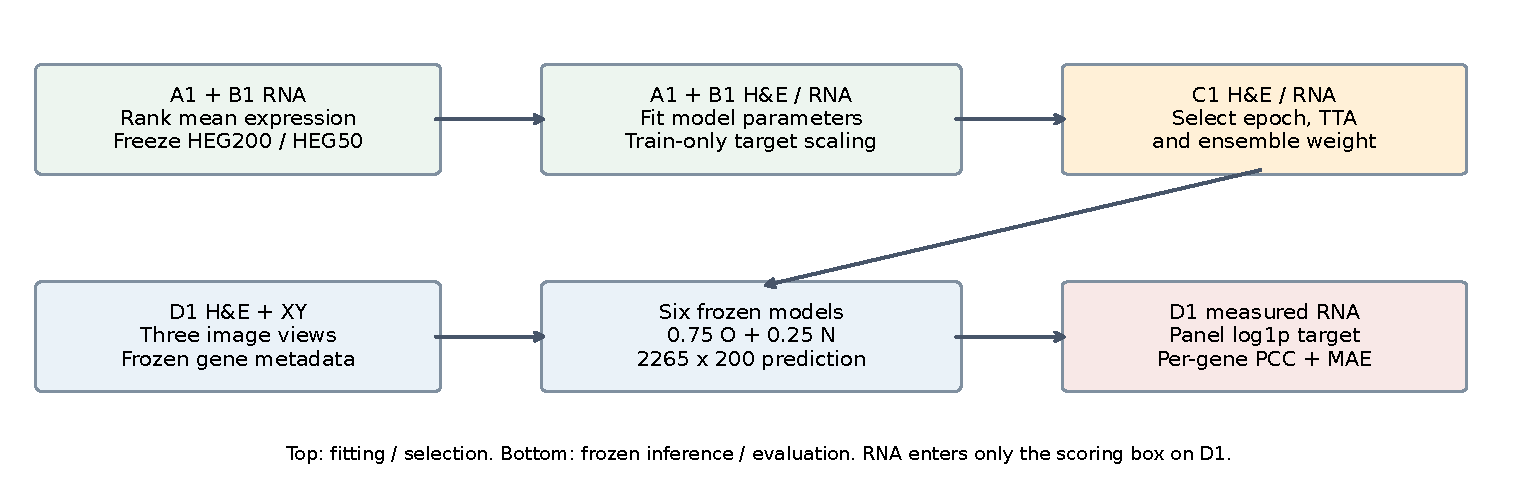
\includegraphics[width=\textwidth]{protocol_flow.pdf}
\caption[从数据划分到预测评价的实验流程]{实验流程。训练集提供图像与表达的配对样本；验证集用于选择网络参数保存时点和集成权重。测试时由图像和位置坐标生成表达预测，随后与 D1 实测 RNA 比较。图中 HEG200/HEG50 指训练集预先选定的两组基因。}\label{fig:protocol}
\end{figure}


\clearpage
\section{预测方法}
\subsection{已有方法及人肝适配范围}
本研究保留五种已有方法的主要建模机制，同时将数据接口、预测基因和输出评价统一到当前任务。不同方法的编码器、训练目标和计算预算仍有差异，因而本实验属于同任务适配比较。以下架构图来自原论文或作者代码仓库，用于解释方法原理；具体适配设置见本节及附录\ref{app:implementation}。

\needspace{12\baselineskip}
\subsubsection{ST-Net：局部图像回归}
ST-Net 使用卷积神经网络提取一个位置周围的图像特征，再通过回归层预测多个基因的表达（图\ref{fig:stnet}）。本研究采用 ImageNet 初始化的 DenseNet121，并将输出层调整为 200 维，在 A1+B1 上微调全部网络参数。它提供了直接从单个局部图块预测表达的端到端参照。

\begin{figure}[H]\centering
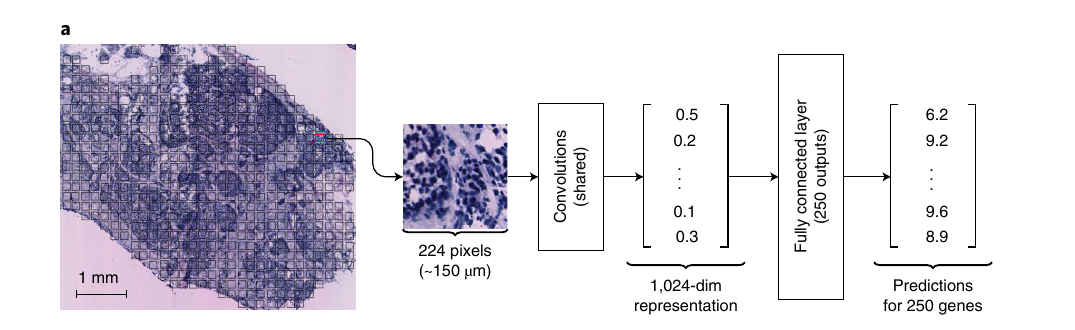
\includegraphics[width=.95\textwidth]{stnet_arch.png}
\caption[ST-Net 的局部图像回归结构]{ST-Net 原论文 Fig. 1a\cite{stnet}。局部图像依次经过卷积编码器和全连接层，得到多基因表达预测。原图输出 250 个基因，本研究的适配实现输出 200 个基因。}\label{fig:stnet}
\end{figure}

此外设置两种简单图像基线：Image Ridge 在固定的 ResNet18 图像特征上训练带正则化的线性回归；MLP 使用两层全连接网络学习同一特征到表达的非线性映射。这两者的图像编码器不更新，与端到端训练的 ST-Net 区分。
\clearpage
\subsubsection{BLEEP：图像与表达对齐后检索}
BLEEP 为图像和表达分别建立编码分支，通过对比学习使同一位置的两个表示在特征空间中接近。预测时，以新图像的表示查询训练集参考库，将相近参考位置的表达组合为输出（图\ref{fig:bleep}）。这一过程利用了训练表达之间的共同结构。

\begin{figure}[H]\centering
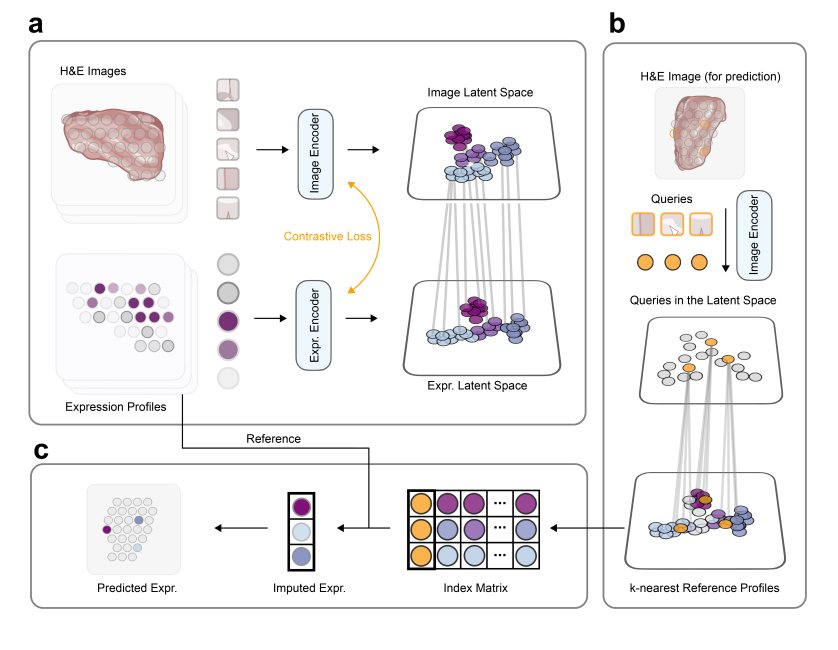
\includegraphics[width=.82\textwidth]{bleep_arch.png}
\caption[BLEEP 的对比学习与表达检索流程]{BLEEP 作者仓库的模型总览\cite{bleep}。训练时将配对图像和表达映射到同一特征空间；预测时根据查询图像检索训练参考表达，并组合成预测表达。参考库仅包含训练切片。}\label{fig:bleep}
\end{figure}

本地适配使用固定的 ResNet18 特征和作者的双投影头，训练图像与表达之间的对齐关系。验证集用于联合选择训练轮次和检索邻居数，最终取第 40 轮、100 个参考邻居。原论文使用的图像编码器和训练预算与此不同，表中结果对应本地适配版本。

\clearpage
\subsubsection{ResSAT：融合形态和空间位置}
ResSAT 同时编码局部图像和二维坐标。Fourier 特征映射把坐标转换为不同频率的正弦、余弦表示，以表达位置变化；特征线性调制（FiLM）再根据坐标分支的输出，对图像特征逐维缩放和平移。注意力模块随后在不同位置之间交换信息（图\ref{fig:ressat}）。与独立预测每个图块相比，该设计能够使用空间关系。

\begin{figure}[H]\centering
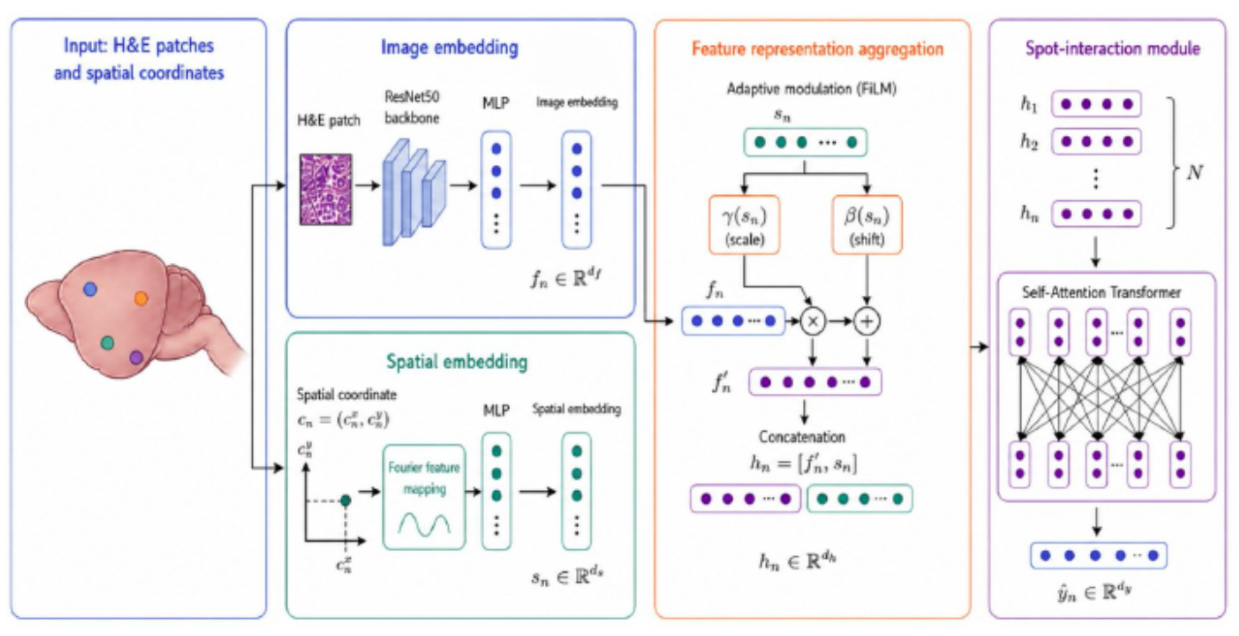
\includegraphics[width=\textwidth]{ressat_arch.png}
\caption[ResSAT 的图像与空间信息融合结构]{ResSAT 2026 接收稿 Fig. 9\cite{ressat}。图像特征与坐标特征分别编码，坐标分支通过 FiLM 调制图像特征，再由注意力模块聚合不同位置的信息。图中展示原作者结构。}\label{fig:ressat}
\end{figure}

本研究复用作者模型主体，将预测基因限制为 HEG200。训练表达先投影到仅由 A1+B1 拟合的 50 维 PCA 空间，即用 50 个主要变化方向表示 200 个基因的表达；预测后再反投影为 200 维表达。训练批大小设为 16，评价采用对应批大小的预测。最终测试参照不经 PCA 重建，因此本实验分数与论文中采用重建表达的结果分别讨论。

\clearpage
\subsubsection{GenAR：逐尺度生成表达}
GenAR 将基因组织为从粗到细的层次，先预测较粗粒度的表达，再利用已有结果预测更细粒度的表达。图像与坐标共同构成生成条件（图\ref{fig:genar}）。这里的“尺度”指表达生成的粒度，与后文三个图像视野的尺度含义不同。

\begin{figure}[H]\centering
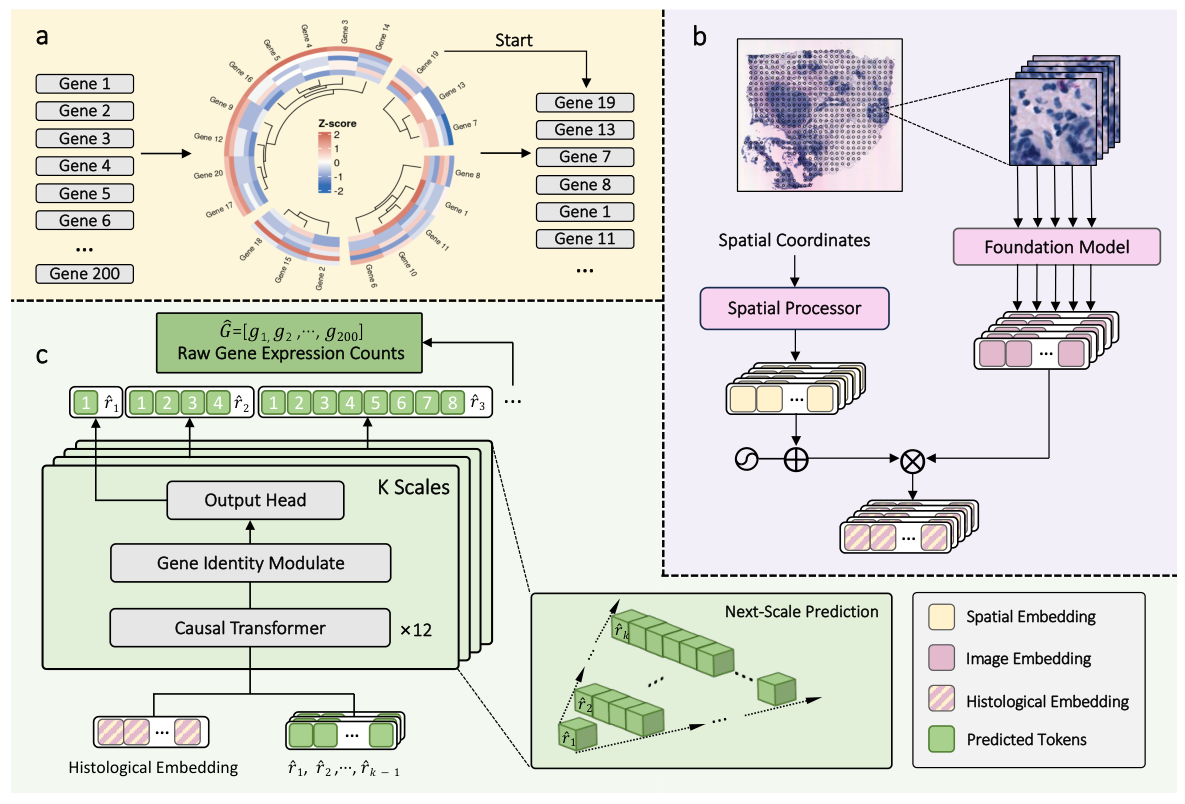
\includegraphics[width=.90\textwidth]{genar_arch.png}
\caption[GenAR 的多尺度自回归结构]{GenAR 预印本 Fig. 1\cite{genar}。(a) 基因按层次组织；(b) 图像特征和空间坐标形成条件表示；(c) 模型依次预测由粗到细的表达，并将前一尺度的结果作为后一尺度的输入。}\label{fig:genar}
\end{figure}

本地实验使用 ResNet18 图像特征，将表达计数编码为离散类别（token），计数上限为 2000。现有训练记录完成 40 轮，所用权重依据训练损失保存；随后在 C1 比较末级解码方式，对概率最高的 8 个计数类别重新归一化概率，再求计数的加权均值，中间尺度仍取最高概率类别。该输出可以为小数。权重保存和解码选择采用不同准则，均在实验记录中保留。

\clearpage
\subsubsection{Stem：图像条件扩散生成}
Stem 通过扩散模型学习图像条件下的表达分布。训练时向表达表示中加入噪声，让网络学习噪声预测；推理时从噪声出发，通过多步更新生成表达。图\ref{fig:stem}给出了两个阶段的数据流。

\begin{figure}[H]\centering
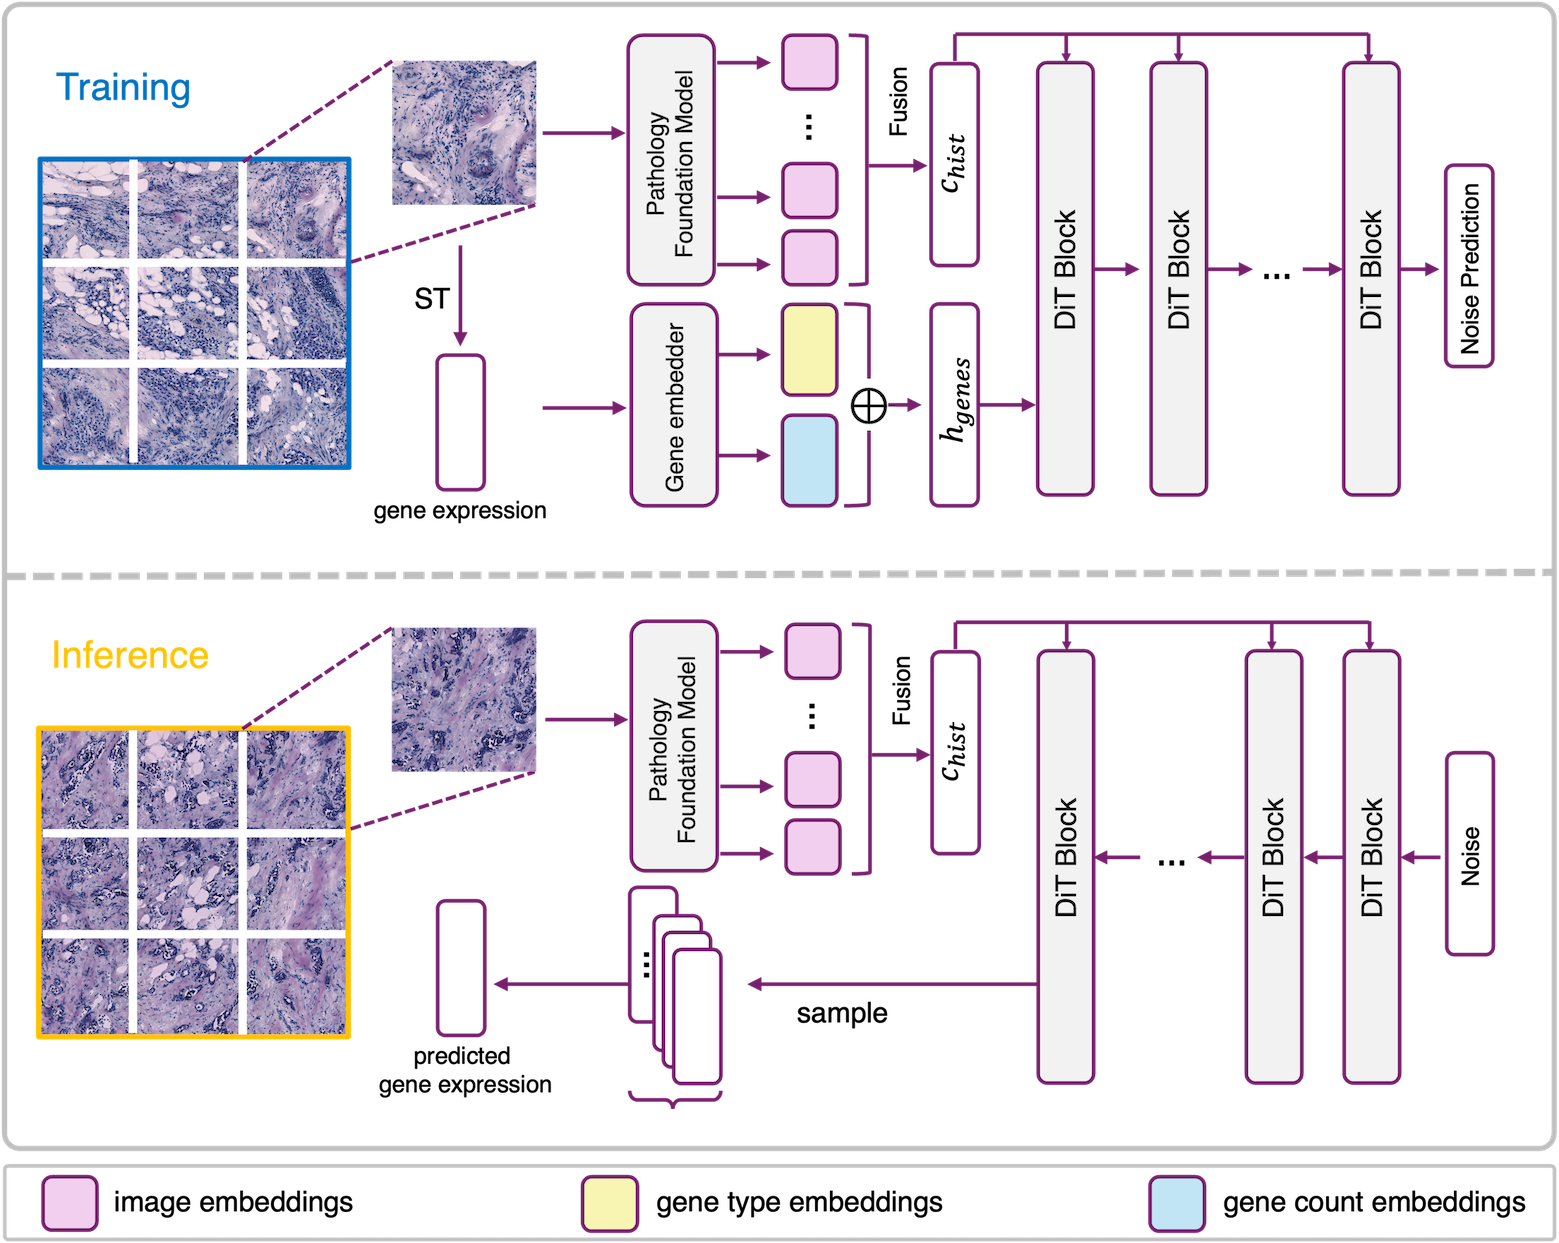
\includegraphics[width=.82\textwidth]{stem_arch.png}
\caption[Stem 的条件扩散训练与推理流程]{Stem 作者仓库 Fig. 1\cite{stem}。上半部分为噪声预测训练，下半部分为从噪声逐步生成表达的推理过程。组织图像特征为两个阶段共同使用的条件信息。}\label{fig:stem}
\end{figure}

本地适配保留作者的扩散 Transformer（DiT）模型，以 ResNet18 特征替代原方法的 UNI 和 CONCH 特征，监督目标采用 200 基因的归一化 log 表达。训练共运行 85 轮，使用第 60 轮保存的模型；推理采用 DDIM 采样器完成 100 步逐步去噪，并平均三次采样的表达。图像条件和训练资源的差异在比较结果时予以考虑。

\clearpage
\subsection{ContextFusion：融合三个图像视野}\label{sec:context}
肝组织的表达变化可能同时对应局部细胞形态与较大范围的组织结构。仅使用与一个 spot 大小接近的图块，可能遗漏周围组织提供的信息。为同时保留两类信息，构建三尺度回归模型 ContextFusion。

对同一 spot，在原始图像上裁取边长为 224、896 和 1792 像素的三个正方形区域，约对应 58、231 和 461 微米。越界部分补白，较大区域经双线性插值缩小至 $224\times224$ 像素。三个输入均为 RGB 图像，使用相同的 ImageNet 通道均值与标准差归一化。位置坐标用于确定裁图中心，不作为该网络的额外数值输入。

\begin{figure}[H]\centering
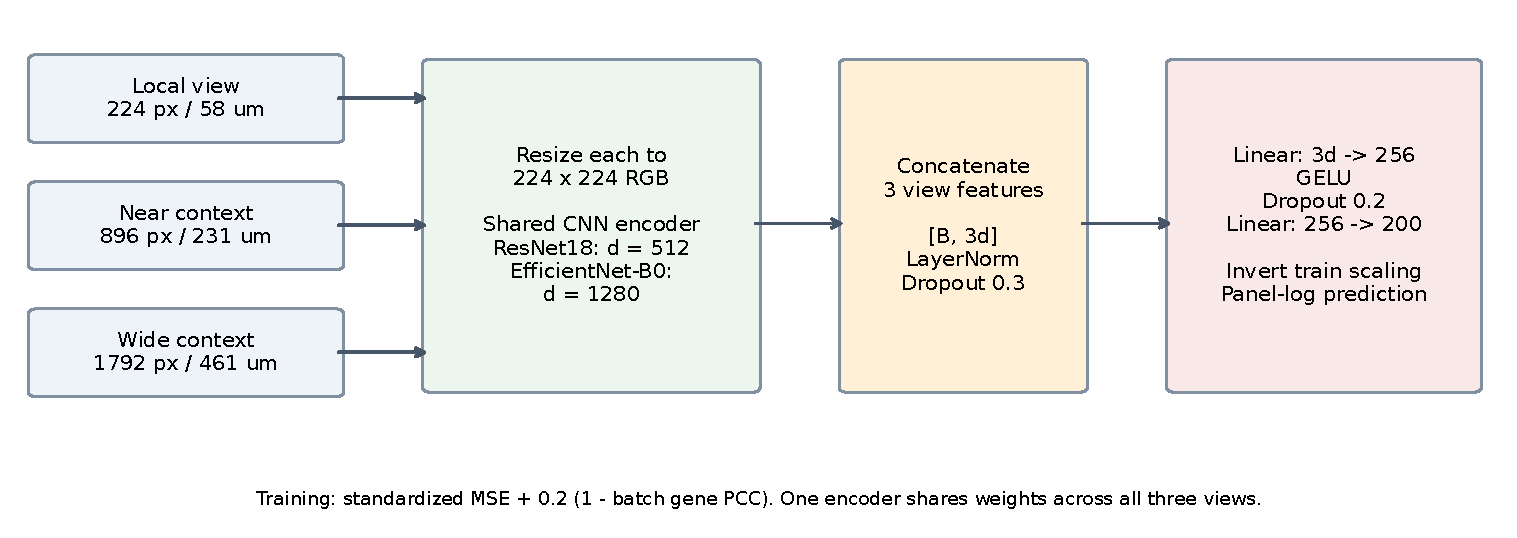
\includegraphics[width=\textwidth]{contextfusion_arch.pdf}
\caption[ContextFusion 三尺度网络]{ContextFusion 网络结构。三个视野经过同一个卷积编码器，特征拼接后由两层回归网络输出 200 个基因的标准化表达。推理末端利用训练集均值和标准差恢复表达单位。}\label{fig:context}
\end{figure}

三个视野通过\textbf{共享参数}的卷积编码器，分别得到特征向量，然后拼接。ResNet18 的每个向量为 512 维，拼接后为 1536 维；EfficientNet-B0 的对应维数为 1280 和 3840。拼接特征依次经过 LayerNorm、Dropout（0.3）、256 维全连接层、GELU、Dropout（0.2）和 200 维输出层。其中 LayerNorm 用于特征归一化，Dropout 在训练中随机屏蔽部分特征以减轻过拟合，GELU 提供非线性变换。编码器与回归层在训练中共同更新。

\begin{figure}[H]\centering
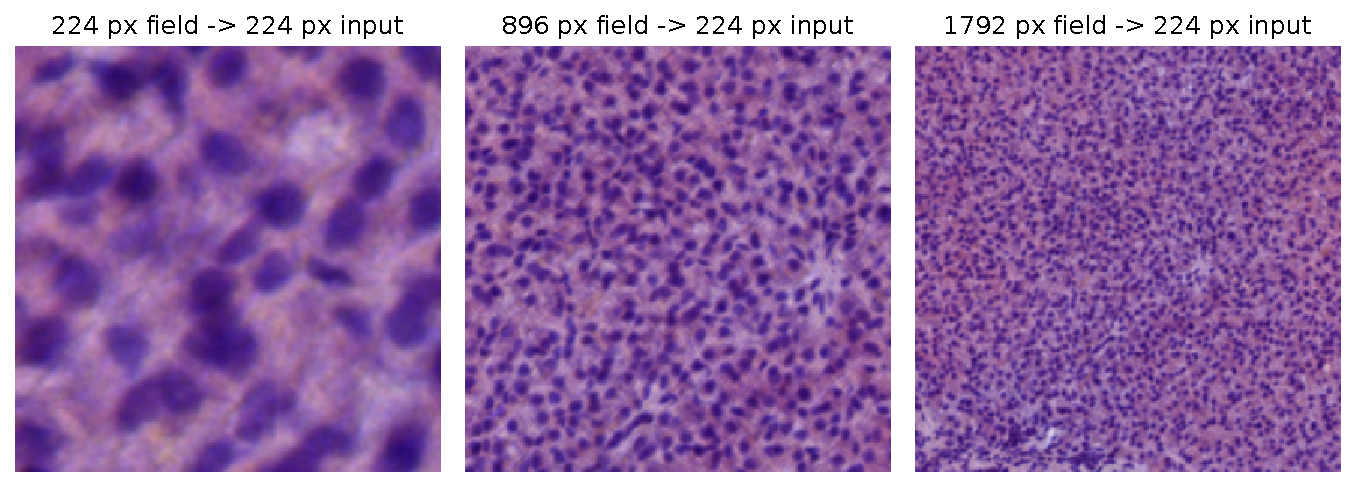
\includegraphics[width=\textwidth]{multiscale_patches.pdf}
\caption[同一位置的三尺度图像输入]{A1 中同一位置的三个实际输入视野。选取距该切片坐标中位数最近的位置作为示例。原始边长分别为 224、896、1792 像素，均缩放到 $224\times224$；由左向右可见组织范围扩大、单个细胞的相对尺寸减小。}\label{fig:patches}
\end{figure}

图\ref{fig:patches}说明，多尺度输入并非将同一小图简单放大，而是从原图提取不同范围的组织。局部图块保留细胞细节，大视野补充组织分布，融合层学习如何利用三种信息。

\subsection{ContextFusion 的训练与模型选择}\label{sec:training}
\subsubsection{监督目标和损失函数}
为了避免高数值范围的基因主导优化，使用训练集统计量逐基因标准化目标。设 $\mu_g$ 为训练均值，$s_g$ 为训练标准差与 0.1 中的较大值，则 $\tilde y_{ig}=(y_{ig}-\mu_g)/s_g$。网络输出 $\tilde{\hat y}_{ig}$，推理时按 $\hat y_{ig}=s_g\tilde{\hat y}_{ig}+\mu_g$ 恢复表达单位。

损失由标准化均方误差和批内相关损失组成：
\begin{equation}
\mathcal L=\frac{1}{B|\mathcal G_{200}|}\sum_{i,g}(\tilde y_{ig}-\tilde{\hat y}_{ig})^2
+0.2\left(1-\frac{1}{|\mathcal G_{200}|}\sum_g r_g^{\rm batch}\right),
\end{equation}
其中 $B$ 为一次参数更新使用的位置数，即批大小；$r_g^{\rm batch}$ 是基因 $g$ 在当前批次位置间的相关系数。第一项约束数值误差，第二项鼓励预测与实测表达的变化方向一致。实现中对相关系数分母加入小常数，以保持低方差批次的数值稳定。

\subsubsection{基础组与扩展组}
为使模型名称对应明确的实验设置，将用于集成的六个模型分为两组。\textbf{基础组}采用同一 ResNet18 结构及训练方案，仅改变随机种子（42、17、83）。随机种子控制参数初始化和训练样本顺序等随机过程；每个模型独立训练。\textbf{扩展组}包含 ResNet18、EfficientNet-B0 和训练标签平滑 ResNet18，三者均使用种子 42。两组均采用 ImageNet 预训练初始化，再更新全部网络参数。


\begin{table}[H]\centering\small
\caption{ContextFusion 两组训练配置}\label{tab:training}
\begin{tabularx}{\textwidth}{lYY}\toprule
设置&基础组&扩展组\\\midrule
优化器&AdamW&AdamW\\
编码器／回归层学习率&$3\times10^{-5}$／$3\times10^{-4}$&$3\times10^{-5}$／$3\times10^{-4}$\\
批大小&24&ResNet18 为24；B0 为16\\
权重衰减&0.01&0.02\\
最大训练轮数&60&45\\
早停条件&验证表现连续12轮未改善&验证表现连续10轮未改善\\
学习率调整&固定学习率&2轮预热后余弦衰减\\
增强方式&旋转、翻转、轻度亮度及对比度变化&旋转、翻转、各通道轻度颜色变化\\
参数平均&不使用&比较当前参数与 EMA 参数\\\bottomrule
\end{tabularx}
\end{table}

一轮训练表示遍历一次训练样本。早停用于在验证表现不再改善时结束训练，而实际用于推理的参数来自验证表现最好的保存时点。扩展组的学习率预热从较小步长开始，余弦调度的下限为初始学习率的 10\%；梯度范数上限为 5，GPU 计算采用 BF16 混合精度。

EMA（exponential moving average，指数移动平均）对训练过程中的网络参数进行平滑平均，扩展组的衰减上限为 0.99。每轮分别评价当前参数和 EMA 参数，并据 C1 的 HEG200 PCC 保存模型。训练标签平滑模型将自身目标与同一训练切片最近 6 个其他位置的目标均值按 0.8 与 0.2 混合；验证和测试目标均保持原值。三组扩展模型实际运行 18、21、18 轮，训练循环分别耗时约 370、837、367 秒。

保存模型后，再比较单次推理与测试时增强（test-time augmentation，TTA）。TTA 分别将图像旋转 $0^\circ$、$90^\circ$、$180^\circ$、$270^\circ$ 输入同一模型，再对四次表达预测取均值。是否使用 TTA 仍依据 C1 的 HEG200 PCC 决定。图\ref{fig:curves}给出扩展组的逐轮验证记录。

\begin{figure}[htbp]\centering
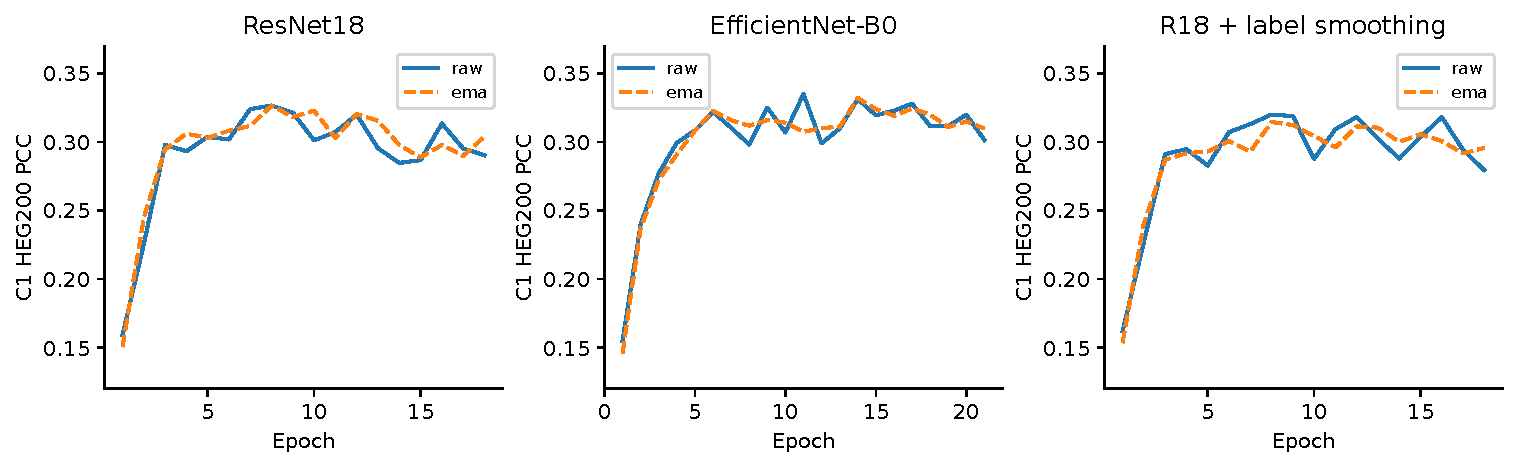
\includegraphics[width=\textwidth]{validation_curves.pdf}
\caption[三个扩展模型的验证集学习曲线]{扩展组模型逐轮验证结果。实线为当前参数，虚线为指数移动平均参数；纵轴均为 C1 的 HEG200 PCC。曲线采用单次推理，保存模型后再评估四旋转平均，因此最终模型选择表中的数值可能略高于曲线峰值。}\label{fig:curves}
\end{figure}


\subsection{六模型加权集成}\label{sec:ensemble}
集成在每个位置、每个基因上对多个模型的预测表达取加权平均。不同随机种子可产生略有差异的拟合结果，不同编码器与训练配置则提供额外预测差异。组合这些输出的目的，是减少单个模型特有的预测波动。

设基础组三个模型的预测矩阵为 $f_{42}$、$f_{17}$、$f_{83}$，扩展组的三个矩阵为 $g_R$、$g_E$、$g_S$。两组内分别等权平均：
\begin{equation}
O=\frac{f_{42}+f_{17}+f_{83}}{3},\qquad
N=\frac{g_R+g_E+g_S}{3}.
\end{equation}
在验证集上，先比较扩展组的三个单模型及其等权平均，选中组平均 $N$；随后将其与 $O$ 按不同权重组合：
\begin{equation}
\hat Y_\alpha=(1-\alpha)O+\alpha N,\quad
\alpha\in\{0,0.25,0.5,0.75,1\}.
\end{equation}
C1 的 HEG200 PCC 在 $\alpha=0.25$ 时最高，故测试使用
\begin{equation}\label{eq:ensemble}
\hat Y_{\rm final}=0.75O+0.25N
=\frac{f_{42}+f_{17}+f_{83}}{4}+\frac{g_R+g_E+g_S}{12}.
\end{equation}
因此，每个基础模型的最终权重为 $1/4$，每个扩展模型为 $1/12$。例如，对某位置的某基因，若基础组平均预测为 4.0，扩展组为 4.4，则集成预测为 $0.75\times4.0+0.25\times4.4=4.1$。该运算直接作用于相同单位的 log 表达，而非平均模型的 PCC 分数。

\begin{figure}[H]\centering
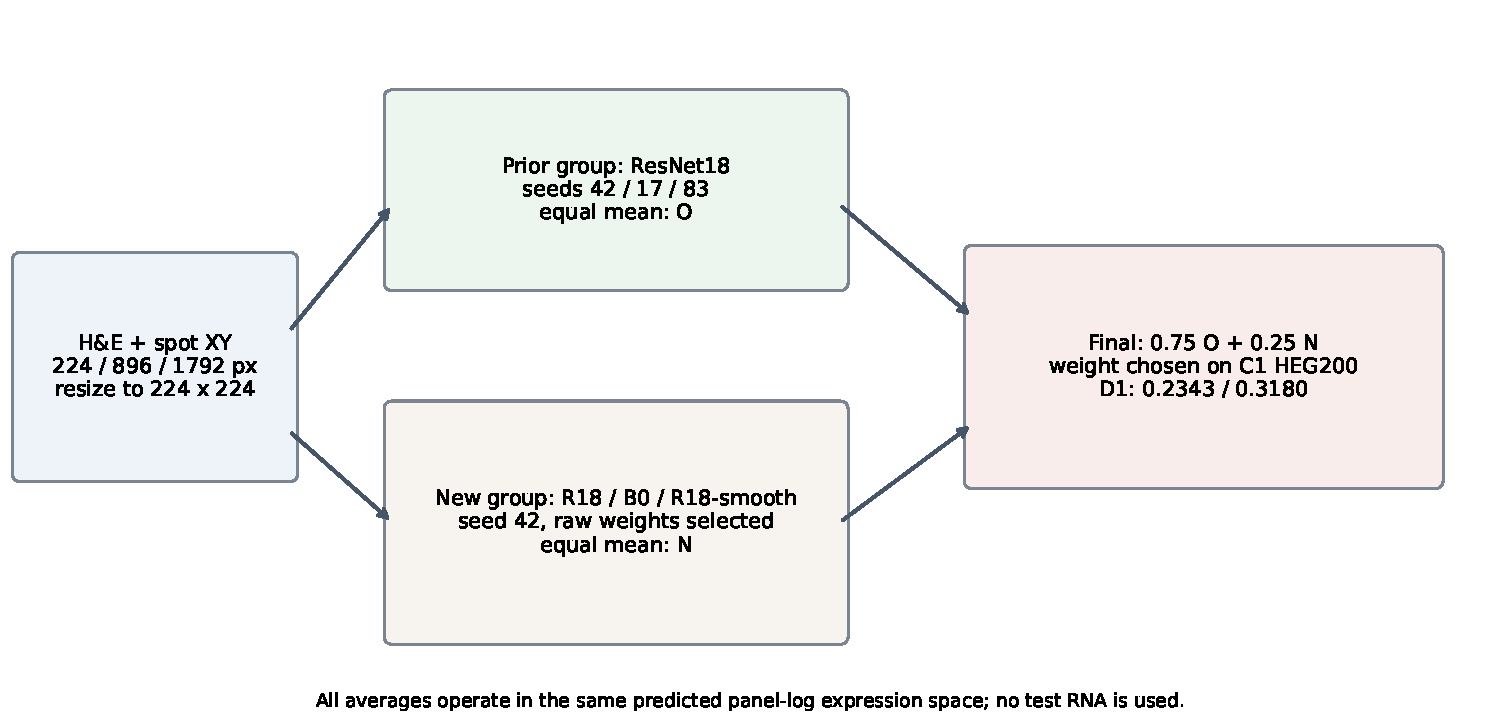
\includegraphics[width=\textwidth]{ensemble_method.pdf}
\caption[六模型集成的组成及预测流程]{六模型集成。基础组包含三个不同随机种子的 ResNet18，扩展组包含 ResNet18、EfficientNet-B0 和训练标签平滑 ResNet18。组内等权平均，组间权重由 C1 选定为 0.75 和 0.25；D1 预测使用同一组权重。}\label{fig:ensemble}
\end{figure}


\begin{table}[H]\centering\small
\caption{六个组成模型的保存轮次、推理方式与权重}\label{tab:components}
\begin{tabular}{lrrr}
\toprule
组成模型 & 保存轮次 & 推理方式 & 最终权重 \\
\midrule
基础组 ResNet18 / seed42 & 9 & 单次 & 1/4 \\
基础组 ResNet18 / seed17 & 9 & 单次 & 1/4 \\
基础组 ResNet18 / seed83 & 19 & 四旋转 & 1/4 \\
扩展组 ResNet18 & 8 & 四旋转 & 1/12 \\
扩展组 EfficientNet-B0 & 11 & 四旋转 & 1/12 \\
训练标签平滑 ResNet18 & 8 & 单次 & 1/12 \\
\bottomrule
\end{tabular}
\end{table}

表\ref{tab:components}列出实际使用的六份模型。所有基因共用式\eqref{eq:ensemble}中的权重；D1 表达不参与权重估计。各模型及组合在验证集和测试集上的完整结果见附录\ref{app:configurations}。

\section{实验设计}
\subsection{方法比较与对照设置}
表\ref{tab:design}概括各项实验的目的和操作。所有人肝主结果使用第2节的数据划分、基因集合和评价指标。

\begin{table}[H]\centering\small
\caption{主要实验及其比较对象}\label{tab:design}
\begin{tabularx}{\textwidth}{>{\raggedright\arraybackslash}p{2.8cm}YY}\toprule
实验&具体操作&回答的问题\\\midrule
已有方法比较&训练或适配七种基线，在 D1 评价&相同数据任务下，各类方法的预测表现如何\\
输入视野对照&以同一局部图块重复三次，替代三个不同视野&保持网络参数量与训练流程后，额外上下文是否有用\\
随机初始化对照&编码器与预测头全部随机初始化并训练&不使用 ImageNet 初始参数时，能否学习人肝表达信号\\
模型集成&比较单模型、基础组平均及六模型组合&不同模型的预测能否互补\\
空间表达分析&绘制固定基因空间图，并比较逐基因 PCC&平均指标的变化对应哪些预测现象\\\bottomrule
\end{tabularx}
\end{table}


输入视野对照使用与基础组种子42模型相同的结构、优化器和损失函数，仅把 896 与 1792 像素视野替换为同一个 224 像素图块的副本。这样保留三路输入及参数量，使差值主要反映额外视野的信息作用。

随机初始化对照不加载预训练参数，编码器和回归头均从随机值开始优化。其编码器学习率为 $3\times10^{-4}$，高于预训练模型的 $3\times10^{-5}$，回归头学习率相同。因此这一对照评价的是可运行的从零训练方案，包含初始化与适配学习率的共同变化。

\subsection{区间估计与空间可视化}
空间位置之间存在相关性。为估计当前测试切片内部的指标波动，将 D1 坐标范围划分为 $5\times5$ 网格，得到 24 个非空空间块。对空间块进行 300 次有放回抽样，每次计算 PCC。比较两个模型时使用相同抽样块，取差值分布的第 2.5 和第 97.5 百分位作为 95\% 区间。该空间块 bootstrap 反映单张切片内的抽样变化，不包含独立患者差异和全部模型选择不确定性。

空间图选用既有分析中的 ALB 和 HP。将每个位置的实测或预测表达赋予颜色，并放回其原始坐标。相同基因的不同方法共用色标，以便观察表达高低区域与动态范围；基因选择不随本次集成结果调整。

\section{实验结果}\label{sec:results}
\subsection{统一人肝任务上的方法比较}
表\ref{tab:main}显示，多尺度六模型集成在本地七种基线适配方法之上取得更高的相关性。HEG200 PCC 为 0.2343，HEG50 为 0.3180；相对其中表现较好的 ST-Net，绝对增量分别为 0.0872 和 0.1202。MAE 从 ST-Net 的 0.4378 降至 0.4274，表明与该参照相比，相关性和数值误差均有改善。

\begin{table}[H]\centering\small
\caption{已有方法适配与六模型集成在 D1 上的比较}\label{tab:main}
\begin{tabular}{lrrr}
\toprule
方法 & HEG200 PCC & HEG50 PCC & MAE \\
\midrule
Image Ridge & 0.0787 & 0.1372 & 0.4490 \\
MLP & 0.0582 & 0.1190 & 0.4714 \\
BLEEP & 0.0915 & 0.1571 & 0.4407 \\
ResSAT & 0.1226 & 0.1846 & 0.4393 \\
GenAR & 0.0492 & 0.1310 & 0.4555 \\
Stem & 0.0668 & 0.1183 & 0.4746 \\
ST-Net (DenseNet121) & 0.1472 & 0.1978 & 0.4378 \\
\textbf{最终六模型集成} & \textbf{0.2343} & \textbf{0.3180} & \textbf{0.4274} \\
\bottomrule
\end{tabular}

\end{table}

这里的差异反映当前完整方案的效果，包含输入视野、编码器和训练策略等共同因素。不同方法的特征来源与预算不完全相同，因此对额外视野的单独作用进一步采用下节的控制实验分析。

\subsection{多尺度输入带来的收益}
在保持模型参数量与训练流程一致的视野对照中，单视野模型的 HEG200/HEG50 PCC 为 0.1941/0.2790，三尺度种子42模型提高到 0.2176/0.3019，增量约为 0.0236/0.0228（表\ref{tab:ablation}）。这一结果支持在局部细胞形态之外，加入周围组织信息有助于当前预测任务。

\begin{table}[H]\centering\small
\caption{图像视野、初始化和集成对照}\label{tab:ablation}
\begin{tabular}{lrrr}
\toprule
方法 & HEG200 PCC & HEG50 PCC & MAE \\
\midrule
三尺度 ResNet18（预训练） & 0.2176 & 0.3019 & 0.4331 \\
三尺度 ResNet18（随机初始化） & 0.2302 & 0.3278 & 0.4197 \\
单视野控制（预训练） & 0.1941 & 0.2790 & 0.4378 \\
基础组三模型集成 & 0.2302 & 0.3156 & 0.4256 \\
最终六模型集成 & 0.2343 & 0.3180 & 0.4274 \\
\bottomrule
\end{tabular}

\end{table}

全随机初始化模型同样获得正向预测相关，HEG200/HEG50 为 0.2302/0.3278，说明当前网络能够从训练图像与表达配对中学习到信号。其 HEG50 高于六模型集成；最终集成方案依据 C1 的 HEG200 选择，因而不是逐项挑选 D1 最优指标得到的组合。

\begin{figure}[H]\centering
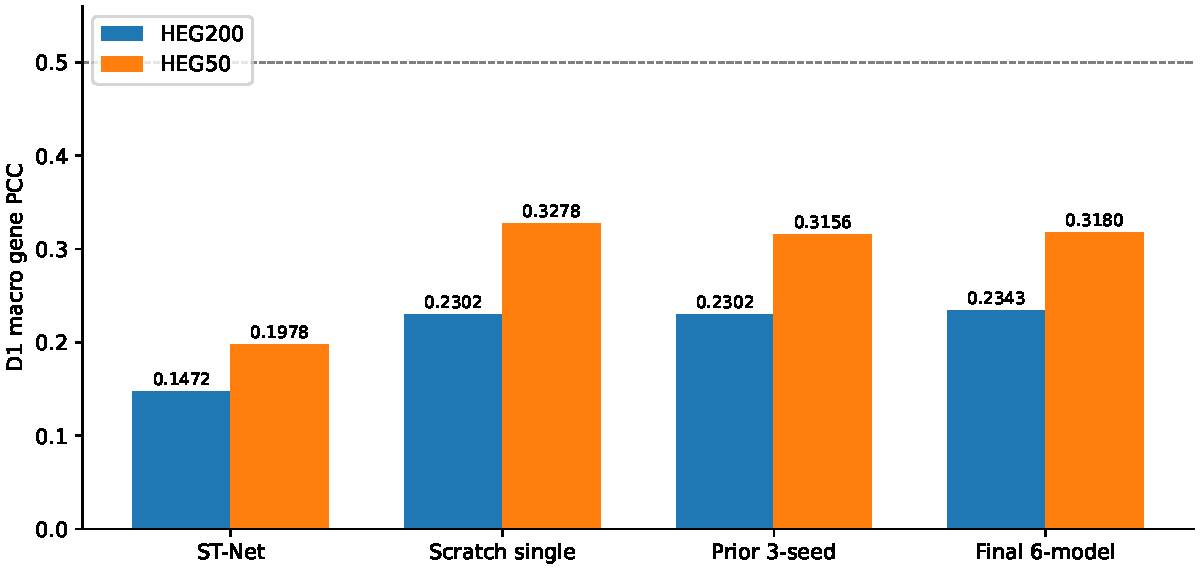
\includegraphics[width=.9\textwidth]{comparison.pdf}
\caption[主要模型在 D1 上的预测性能]{主要模型的 D1 宏平均 PCC。蓝色表示 HEG200，橙色表示 HEG50；Scratch single 为全随机初始化的三尺度单模型，Prior 3-seed 为基础组三模型平均。横向虚线仅标示 PCC 为 0.5 的位置。}\label{fig:comparison}
\end{figure}


\subsection{模型集成与逐基因表现}
基础组三个随机种子的预测均值达到 0.2302/0.3156，六模型集成进一步达到 0.2343/0.3180。相对基础组，HEG200 和 HEG50 PCC 分别增加 0.0042 和 0.0024。图\ref{fig:pergene}中的配对比较显示，151 个基因的 PCC 上升、49 个下降，表明平均增益由多个基因共同贡献。

\begin{figure}[htbp]\centering
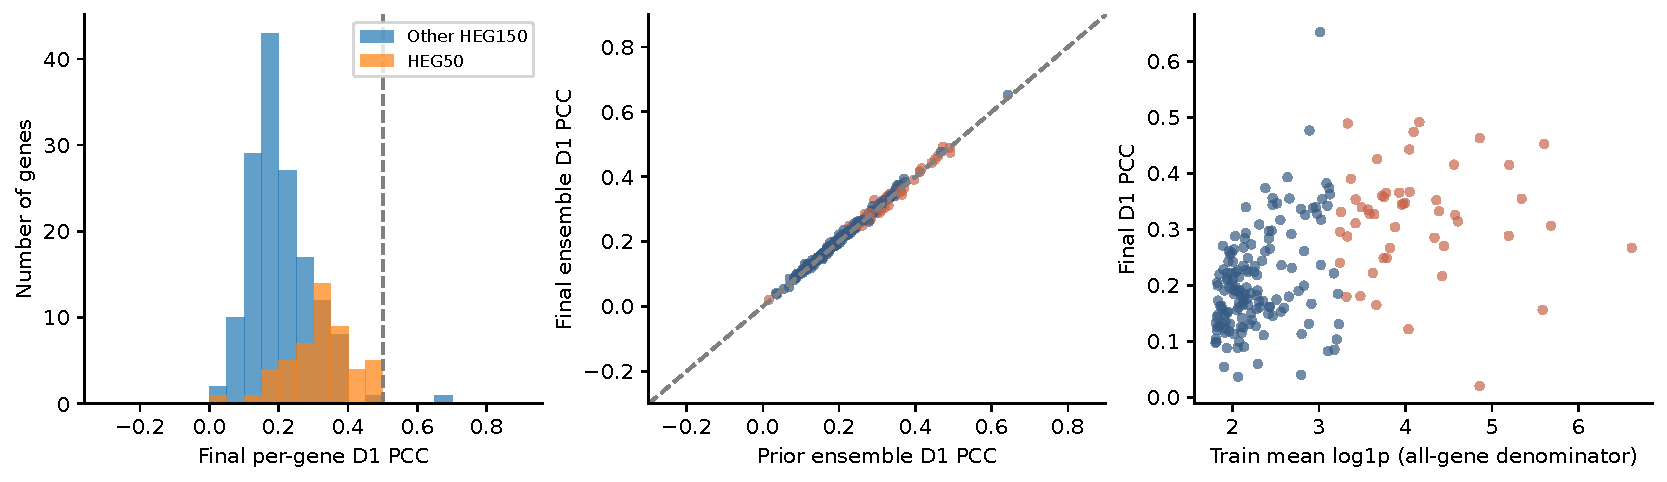
\includegraphics[width=\textwidth]{per_gene_diagnostics.pdf}
\caption[逐基因预测表现及集成前后的变化]{固定 HEG200 的逐基因结果。左：最终 PCC 的分布；中：基础组与六模型集成的配对比较，虚线表示二者相等；右：训练平均表达量与测试 PCC 的关系。橙色表示 HEG50，所有 200 个基因均纳入统计。}\label{fig:pergene}
\end{figure}

训练平均表达与最终测试 PCC 的 Spearman 相关为 0.555，提示高表达基因在当前任务中通常具有较好的预测表现。与此同时，同等表达水平的基因仍存在明显差异，说明表达丰度之外的空间结构与形态关联也需要考虑。该关联分析仅用于解释结果，未参与基因筛选。


\begin{table}[H]\centering\small
\caption{六模型集成的空间块 bootstrap 结果}\label{tab:ci}
\begin{tabular}{lrr}\toprule
指标&点估计&95\%区间\\\midrule
HEG200 PCC&0.2343&[0.1807, 0.2765]\\
HEG50 PCC&0.3180&[0.2489, 0.3722]\\
相对基础组的 HEG200 增量&0.0042&[0.0009, 0.0077]\\
相对基础组的 HEG50 增量&0.0024&[$-0.0037$, 0.0091]\\\bottomrule
\end{tabular}
\end{table}

表\ref{tab:ci}中，HEG200 增量区间高于零，而 HEG50 增量区间包含零。因此，集成收益主要体现为当前切片上小幅的 HEG200 相关性提升。相对基础组，MAE 由 0.4256 增至 0.4274；这一权衡表明相关性改善并不必然降低所有误差指标。

\subsection{预测表达的空间分布}
图\ref{fig:spatial}将平均指标还原为具体基因的空间分布。每个点对应一个测量位置，颜色表示式\eqref{eq:target}的表达值；从左到右可比较实测表达、ST-Net、基础组和最终集成。图中既能观察较大范围的表达高低变化，也能辨认模型之间的数值范围差异。

\begin{figure}[H]\centering
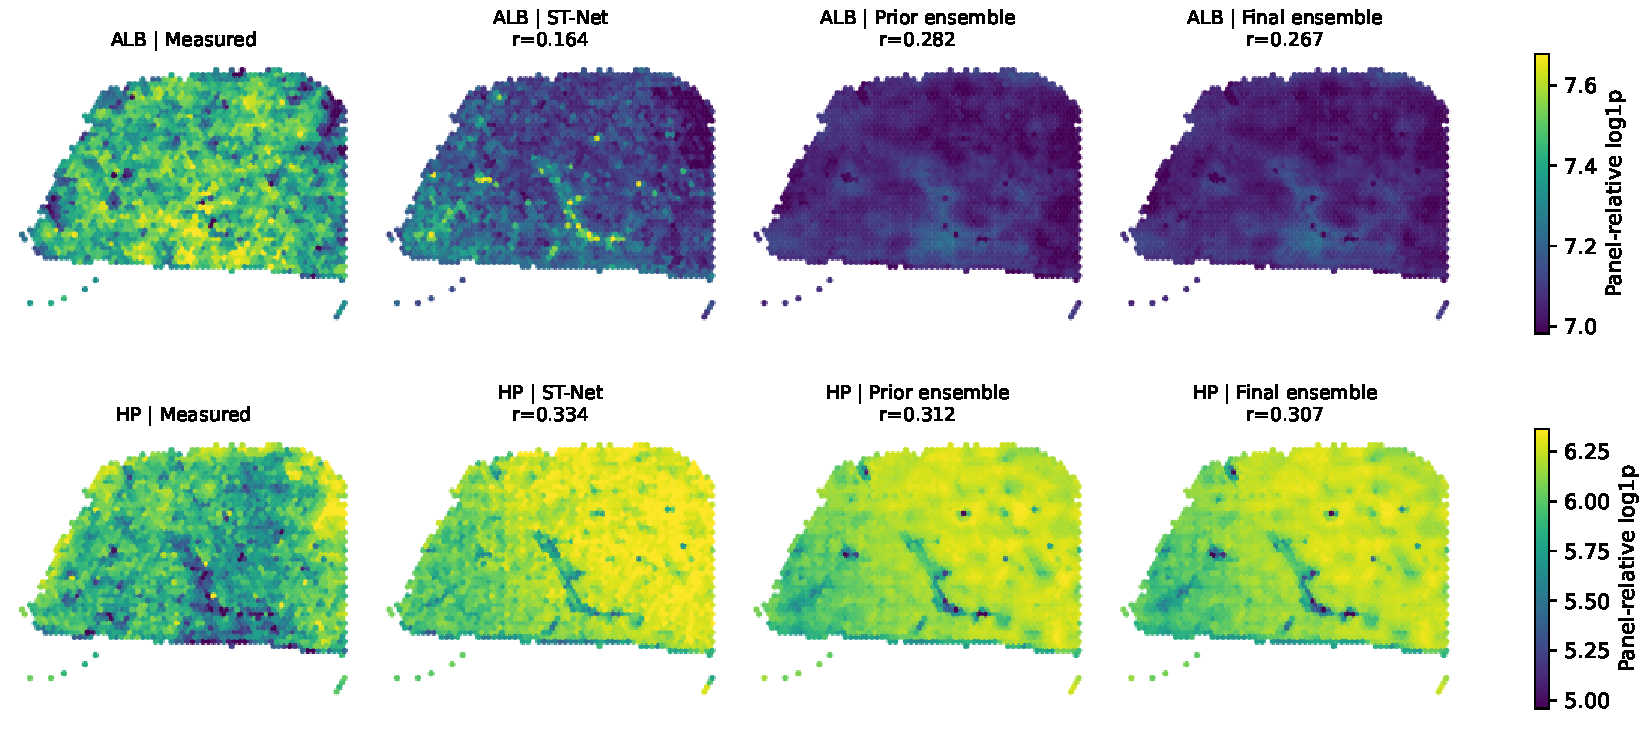
\includegraphics[width=\textwidth]{spatial_examples.pdf}
\caption[ALB 和 HP 的空间表达预测]{ALB、HP 的实测与预测空间表达。每行对应一个基因，各方法共用该基因实测表达第 1 至第 99 百分位的色标；超出范围的颜色截断只影响显示。标题中的 PCC 使用全部数值计算。ALB 与 HP 沿用既有示例，用于观察表达分布，不参与基因集合选择。}\label{fig:spatial}
\end{figure}

空间图与逐基因 PCC 共同用于检查模型是否恢复了表达变化的方向。色彩分布近似并不保证每个位置的数值都准确，因此数值误差仍以 MAE 评价。两例图像作为对整体统计的补充，其表现不外推到全部基因。

\section{讨论}
\subsection{主要改进及其证据}
本研究的改进首先建立在明确的预测目标上：基因按训练平均表达选择，所有方法使用相同测试基因和实测目标。随后通过三尺度输入扩大组织视野，利用端到端训练使图像编码器适应人肝表达任务。严格保持参数量的视野对照获得正向增量，为多尺度设计提供了直接证据。

集成进一步组合不同随机种子和训练配置的输出。其优势在于无需改变测试输入或表达参照，即可在相同基因集合上改善部分预测。当前六模型相对基础组三模型的增益较小，残差相关分析见附录\ref{app:supplement}。因此，主要性能提升应归于完整的多尺度学习方案，集成提供进一步的有限补充。

\subsection{跨切片预测差异的可能来源}
以基础组三尺度种子42模型为例，训练集、C1 和 D1 的 HEG50 PCC 分别约为 0.6082、0.4854 和 0.3019。训练表现高于测试表现，说明模型能够拟合配对信号，但跨切片仍存在分布差异。当前仅两张训练切片，组织形态和染色变化的覆盖范围有限。

表达测量条件也可能影响评价。每个位置的全转录组 UMI 计数中位数在 A1、B1、C1、D1 分别为 8134、6537、12423、6010。UMI 为用于区分捕获转录本的分子标识，其计数同时受生物 RNA 含量和实验捕获过程影响。固定 C1 预测，将其原始计数按约 0.484 的保留概率二项降采样并重复 30 次后，该模型 HEG200 PCC 由 0.3485 降至平均约 0.3033。该代理实验支持计数差异可能贡献部分验证与测试落差，但尚不能分离生物差异、捕获效率和测序过程的各自作用。

\subsection{与原论文结果的关系}
不同研究的 PCC 必须结合组织、基因选择和表达处理理解。ResSAT 文中的 0.6577 和 0.6980 来自鼠脑 2000 个高变基因及 PCA/Harmony 重建表达设置；本地对应单种子重现约为 0.6506 和 0.6667。该实验用于核对方法与评价流程，与本报告的人肝 HEG200 任务分别记录。

同一批人肝切片上，BLEEP 原论文报告 HEG50 PCC 为 $0.175\pm0.016$，后续单图块 EfficientNet-B0 研究报告约 0.310\cite{bleep,singlepatch}。两者使用 slice 3（C1）测试，其余三张训练，并采用四切片高变基因并集及 Harmony 处理。与本研究的训练、验证、测试划分和基因集合不同，这些数值提供同组织的研究背景，但不构成直接排名。单个基因的高 PCC 也不能等同于固定基因集合的平均 PCC。

\subsection{适用范围与后续研究}
当前结果表明，人肝组织图像中包含可用于预测部分基因表达变化的信息。研究仍受单供体、训练切片较少以及方法预算不完全一致的限制，测试基因平均 PCC 尚未达到 0.5。后续应在独立供体上检验模型，并在相同训练预算下比较组织预训练编码器与现有编码器，以确定性能差异能否跨样本保持。

\section{结论}
本研究在明确的训练、验证和测试划分下，完成了从人肝 \HE 图像到 200 个高表达基因空间表达的预测，并比较了五种已有方法的适配实现及图像回归基线。三尺度 ContextFusion 通过联合观察局部细胞形态与周围组织，取得优于单视野对照的结果；六模型加权集成的 D1 HEG200 和 HEG50 PCC 分别为 0.2343 和 0.3180，较本地 ST-Net 适配分别提高 0.0872 和 0.1202。

实验支持将多尺度组织信息用于人肝空间表达预测，并为模型集成的增益范围提供了定量证据。所建立的数据处理、模型选择和结果核验流程可用于后续扩展到更多供体及更大规模的数据。

\clearpage
\appendix
\section{方法适配与复现实验设置}\label{app:implementation}
\subsection{已有方法的训练目标与选择方式}
为便于区分作者方法和本地实现，表\ref{tab:adaptation}概括各方法的主要适配。表内“全转录组 log 目标”指选取的 200 个基因仍以每个位置的全转录组总计数归一化；其预测最终按第\ref{sec:target}节换算。

\begin{table}[H]\centering\footnotesize
\caption{已有方法的实际实现及模型选择}\label{tab:adaptation}
\begin{tabularx}{\textwidth}{>{\raggedright\arraybackslash}p{1.8cm}YY}\toprule
方法&训练与输出&选择或推理设置\\\midrule
Image Ridge&固定 ResNet18 特征；全转录组 log 目标&正则系数候选为1、10、100、1000，以 C1 选择\\
MLP&固定512维特征；256维隐藏层和200维输出；全转录组 log 目标&AdamW，学习率$10^{-3}$，批128；按验证损失早停\\
ST-Net&ImageNet DenseNet121 全参数微调；200维输出；全转录组 log 目标&C1 PCC 选第10轮，使用四旋转平均\\
BLEEP&固定 ResNet18 特征；双投影头与对比损失；参考库表达检索&AdamW，学习率$10^{-3}$，批128；最多120轮；C1联合选择轮次和邻居数\\
ResSAT&作者网络；训练集拟合PCA50；预测后反投影&最多100轮，学习率$5\times10^{-4}$，批16，早停耐心值10\\
GenAR&固定 ResNet18 特征；计数token生成，计数上限2000&批16，学习率$10^{-4}$；完成40轮，权重按训练损失保存；C1选择末级top-8期望解码\\
Stem&固定 ResNet18 条件；DiT 12层、隐藏维384、6头；全转录组 log 目标&AdamW，学习率$10^{-4}$，批32；固定验证噪声，按验证损失保存；DDIM100三次均值\\\bottomrule
\end{tabularx}
\end{table}

ResSAT 的 Fourier 特征数为128、尺度参数为1、Dropout为0.3、权重衰减为$10^{-6}$。Stem 的 EMA 衰减改为0.99，并在 C1 的预定256位置子集上比较当前参数／EMA及采样截断方式，最终使用当前参数和训练范围截断。它与扩展组 ContextFusion 的训练标签平滑是不同操作。

已有方法的模型保存准则并非完全相同。主结果统一测试条件，但不能将所有方法描述为按同一验证 PCC 训练选择，也不能将适配结果等同于原论文计算规模下的复现。

\subsection{数据对齐与执行环境}
表达矩阵按位置条形码（barcode）与坐标对齐，再按统一基因列表确定列顺序。基因列表保留已有 GenAR 层次排序，列表成员仍为训练平均表达前200个基因。四切片的原始计数、归一化表达、基因名、条形码和坐标均完成逐元素核验，144 个跨尺度图块与原图裁取结果一致。

训练主要使用 WSL 全局 Python 3.12.3、PyTorch 2.9.1、torchvision 0.24.1 和 NVIDIA GeForce RTX 5060 Laptop GPU。六份最终模型在2026年9月15日重新推理，得到的 $2265\times200$ 预测矩阵与保存结果逐元素一致。该核验对应当时的硬件和数值配置。

基因文件为 \code{benchmarks/liver/genes.csv}，六模型的路径、权重摘要和推理设置记录于 \code{benchmarks/liver/final_ensemble.json}。模型预测仅需要图像、位置和基因元数据；评价阶段另行读取测试表达。以下命令给出 Bash 下的重推理及评价入口：
\par\noindent\begin{minipage}{\textwidth}\begin{small}\begin{verbatim}
python run.py ensemble --slides C73_D1 \
  --output results/final_prediction.npz
python run.py evaluate \
  --prediction results/final_prediction.npz \
  --truth data/processed/gse240429_heg/arrays/C73_D1.npz \
  --output results/final_metrics.json
\end{verbatim}\end{small}\end{minipage}\par
运行需事先准备数据缓存与六份模型参数。代码仓库保存训练入口、配置和文件摘要，大型原始数据与权重单独保留。

\section{完整配置比较}\label{app:configurations}
表\ref{tab:complete}保留全部既有基线与 ContextFusion 对照，以支持正文的主要比较。Context-RBF 为固定多尺度特征上的径向基核回归；它与端到端 ContextFusion 分别作为特征回归和图像特征学习的方案记录。

\begin{table}[H]\centering\small
\caption{全部基线与结构对照的 D1 结果}\label{tab:complete}
\begin{tabular}{lrrr}
\toprule
方法 & HEG200 PCC & HEG50 PCC & MAE \\
\midrule
Image Ridge & 0.0787 & 0.1372 & 0.4490 \\
MLP & 0.0582 & 0.1190 & 0.4714 \\
BLEEP & 0.0915 & 0.1571 & 0.4407 \\
ResSAT & 0.1226 & 0.1846 & 0.4393 \\
GenAR & 0.0492 & 0.1310 & 0.4555 \\
Stem & 0.0668 & 0.1183 & 0.4746 \\
ST-Net (DenseNet121) & 0.1472 & 0.1978 & 0.4378 \\
多尺度特征核回归 & 0.1327 & 0.1809 & 0.4633 \\
三尺度 ResNet18（预训练） & 0.2176 & 0.3019 & 0.4331 \\
三尺度 ResNet18（随机初始化） & 0.2302 & 0.3278 & 0.4197 \\
单视野控制（预训练） & 0.1941 & 0.2790 & 0.4378 \\
基础组三模型集成 & 0.2302 & 0.3156 & 0.4256 \\
最终六模型集成 & 0.2343 & 0.3180 & 0.4274 \\
\bottomrule
\end{tabular}
\end{table}


表\ref{tab:opt}给出扩展组及其混合权重的全部评价。扩展组25\%对应正文的六模型集成。C1 HEG50 为0.5052，D1为0.3180，两者分别是验证和测试结果。

\begin{table}[H]\centering\footnotesize
\caption{扩展模型与不同组间权重的完整比较}\label{tab:opt}
\begin{tabular}{lrrrrr}
\toprule
候选 & C1/200 & C1/50 & D1/200 & D1/50 & D1 MAE \\
\midrule
扩展组 ResNet18 & 0.3303 & 0.4602 & 0.2182 & 0.2947 & 0.4446 \\
扩展组 B0 & 0.3439 & 0.4779 & 0.2274 & 0.2998 & 0.4324 \\
扩展组平滑 ResNet18 & 0.3200 & 0.4410 & 0.2010 & 0.2635 & 0.4432 \\
扩展组等权平均 & 0.3481 & 0.4799 & 0.2264 & 0.2987 & 0.4369 \\
基础组等权平均 & 0.3626 & 0.5008 & 0.2302 & 0.3156 & 0.4256 \\
六模型集成（扩展组25\%） & 0.3665 & 0.5052 & 0.2343 & 0.3180 & 0.4274 \\
扩展组50\% & 0.3641 & 0.5016 & 0.2342 & 0.3147 & 0.4299 \\
扩展组75\% & 0.3574 & 0.4925 & 0.2311 & 0.3077 & 0.4331 \\
\bottomrule
\end{tabular}
\end{table}

扩展组标签平滑单模型低于对应非平滑模型，三个扩展模型最终均使用当前参数而非EMA。基础组与扩展组同时调整了学习率调度、增强和正则化，因而组间差值不能归因于单一训练因素。全文主要结论建立在同任务比较及单视野控制上。

\section{补充诊断实验}\label{app:supplement}
\subsection{组成模型的残差相关性}
为了了解模型间的误差是否具有互补性，对每个模型计算 $e_m=\hat Y_m-Y$，将全部位置和基因的残差展开为向量，再计算模型两两相关。图\ref{fig:residual}中的非对角相关为0.974--0.992，表明残差高度相似。

\begin{figure}[H]\centering
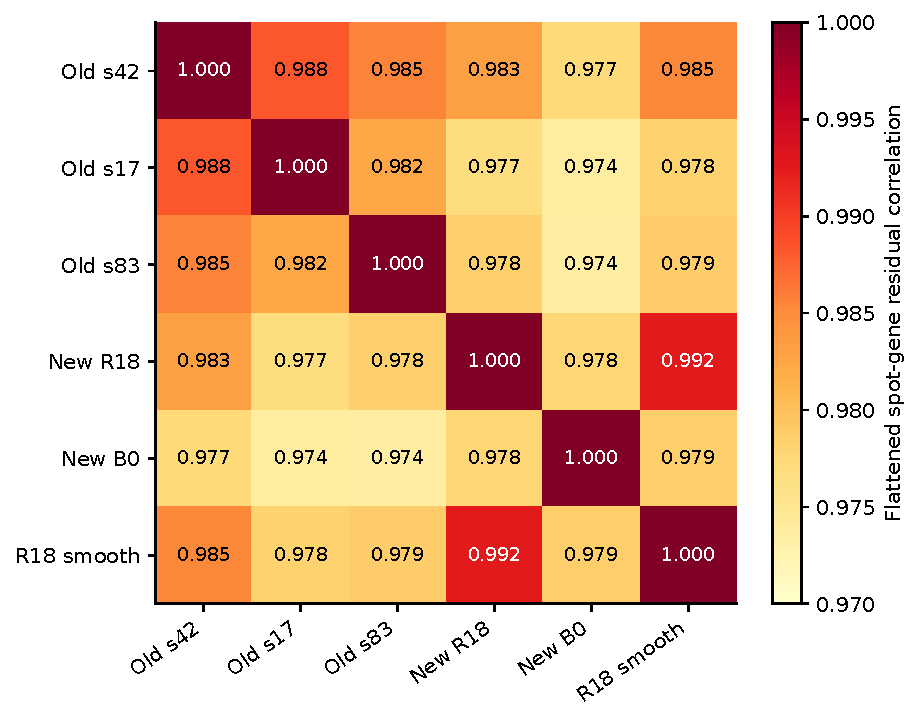
\includegraphics[width=.74\textwidth]{residual_correlation.pdf}
\caption[组成模型的预测残差相关矩阵]{六个模型在 D1 的残差相关性。残差为预测减实测表达，将全部位置和基因展开后计算 Pearson 相关。色标范围为 0.97--1.00。该统计用于分析模型间的误差相似性，不参与集成权重选择。}\label{fig:residual}
\end{figure}

加权平均能够抵消一部分模型特有的波动，但高度共享的误差会限制这一收益。共同测量噪声和基因尺度也会影响残差相关，因此该分析为描述性证据，未用于选择权重或识别单一误差来源。

\subsection{预测空间平滑对照}
为检验局部预测波动能否通过邻域平均减小，以六模型输出为输入，构造
\begin{equation}
\hat y_i^{(k,\alpha)}=(1-\alpha)\hat y_i+
\frac{\alpha}{k}\sum_{j\in\mathcal N_k(i)}\hat y_j.
\end{equation}
$\mathcal N_k(i)$ 是按图像坐标确定、排除自身的 $k$ 个近邻。预设邻居数为6、12、24，混合权重为0.25、0.5、0.75、1，并加入不平滑对照，共13个候选。仅按 C1 HEG200 PCC 选择，模型和实测目标均不改变。

\begin{figure}[H]\centering
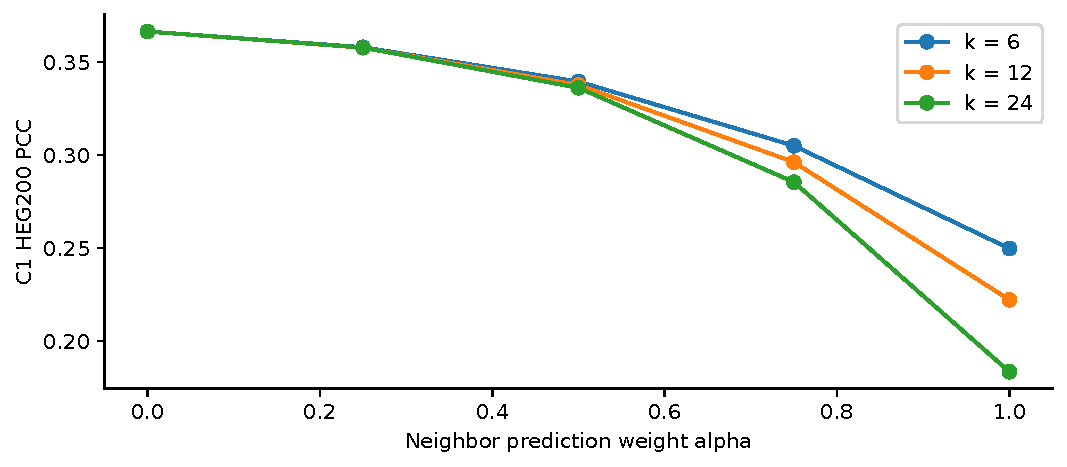
\includegraphics[width=.84\textwidth]{prediction_smoothing.pdf}
\caption[预测空间平滑的验证结果]{预测空间平滑的 C1 结果。横轴为邻域预测的混合权重，$k$ 为参与平均的邻居数。零权重对应未平滑的六模型输出。所有候选使用相同模型与实测目标。}\label{fig:smoothing}
\end{figure}

C1 选择不平滑输出（HEG200为0.3665）；最佳非零平滑候选为$k=6$、$\alpha=0.25$，对应0.3580。因此最终测试预测保持不变。该结果限定于所测试的邻域和权重范围，不扩展为对所有空间建模方法的判断。完整计划、验证结果与选择记录见 \code{benchmarks/liver/report_spatial_ablation/}。

\subsection{预处理核验与论文指标复查}
早期基因列表按表达方差选择并排除了核糖体和线粒体基因，与当前高表达集合没有重叠。现有主表已按第2节重新选择基因并使用一致测试目标，早期列表的分数不用于证明当前模型改进。不同归一化分母引起的指标变化也与同一目标上的模型改进分开记录。

鼠脑 ResSAT 复查采用单种子实验：SA 使用作者处理后示例，SP 根据当前下载数据近似重建处理流程。重建目标下2000个高变基因 PCC 分别为0.6506和0.6667，对应原论文0.6577和0.6980；该设置下高表达50基因的本地结果为0.8803和0.8930。它们验证的是论文相关条件下的结果量级，不纳入人肝方法排序。

\clearpage
\begin{thebibliography}{9}
\addcontentsline{toc}{section}{参考文献}
\bibitem{stnet} He B, Bergenstråhle L, Stenbeck L, et al. Integrating spatial gene expression and breast tumour morphology via deep learning. \textit{Nature Biomedical Engineering}, 2020. \url{https://doi.org/10.1038/s41551-020-0578-x}.
\bibitem{bleep} Xie R, Pang K, Chung S W, et al. Spatially Resolved Gene Expression Prediction from H\&E Histology Images via Bi-modal Contrastive Learning. \textit{NeurIPS}, 2023. \url{https://github.com/bowang-lab/BLEEP}.
\bibitem{ressat} Liu A, Zhao Y, Kim W K, et al. ResSAT: enhancing spatial transcriptomics prediction from H\&E-stained histology images with an interactive spot transformer. \textit{Genome Biology}, 2026, article in press. \url{https://doi.org/10.1186/s13059-026-04168-x}.
\bibitem{genar} Ouyang J, Wang Y, Gao Y, et al. GenAR: Next-Scale Autoregressive Generation for Spatial Gene Expression Prediction. arXiv:2510.04315, 2025. \url{https://arxiv.org/abs/2510.04315}.
\bibitem{stem} Zhu S, Zhu Y, Tao M, Qiu P. Diffusion Generative Modeling for Spatially Resolved Gene Expression Inference from Histology Images. \textit{ICLR}, 2025. \url{https://github.com/SichenZhu/Stem}.
\bibitem{geo} NCBI Gene Expression Omnibus. GSE240429: human liver spatial transcriptomics data. 数据访问与下载记录见项目数据说明。\url{https://www.ncbi.nlm.nih.gov/geo/query/acc.cgi?acc=GSE240429}.
\bibitem{andrews} Andrews T S, Nakib D, Perciani C T, et al. Single-cell, single-nucleus, and spatial transcriptomics characterization of the immunological landscape in the healthy and PSC human liver. \textit{Journal of Hepatology}, 2024, 80(5):730--743. \url{https://doi.org/10.1016/j.jhep.2023.12.023}.
\bibitem{singlepatch} Jang H, Shin H, et al. From histology to spatial transcriptomics: establishing a lightweight single-patch baseline. \textit{BMC Bioinformatics}, 2026, 27:168. \url{https://doi.org/10.1186/s12859-026-06447-7}.
\end{thebibliography}
\end{document}
